\subsection{面积概念和公理}\label{subsec:czjh1-5-1}

在小学里我们学习过一些面积的计算。在日常生活和生产中,会经常遇到面积的问题。
例如,计算土地的面积、住房的面积、各种物体的表面积等。
这些问题都与各种多边形的面积有关,因此.我们需要进一步研究多边形的面积。

\begin{wrapfigure}[8]{r}{8.5cm}
    \centering
    \begin{tikzpicture}
    \begin{scope}[xshift=-2cm]
        \tkzDefPoints{0/0/A, 1/0/B, 1/1/C, 0/1/D}
        \tkzDrawPolygon(A,B,C,D)
        \tkzLabelSegment[below](A,B){$1$}
        \tkzLabelSegment[right](B,C){$1$}
    \end{scope}

    \begin{scope}
        \tkzDefPoints{0/0/A, 7/0/B, 5/4/C, 0/4/D}
        \tkzClipPolygon(A,B,C,D)
        \foreach \x in {0,...,7} {
            \tkzDefPoints{\x/0/X1, \x/4/X2}
            \tkzDrawSegments(X1,X2)
        }
        \foreach \y in {0,...,4} {
            \tkzDefPoints{0/\y/Y1, 7/\y/Y2}
            \tkzDrawSegments(Y1,Y2)
        }
        \tkzDrawPolygon[very thick](A,B,C,D)
    \end{scope}
\end{tikzpicture}


    \caption{}\label{fig:czjh1-5-1}
\end{wrapfigure}

多边形的\zhongdian{面积}, 就是它所围的平面部分的大小。
大小是用数来表示的,要表示一个多边形的面积,和度量线段时一样,必须取一个单位,
然后看这个多边形所围平面部分是单位的多少倍,这个倍数就是面积的数值。
面积的单位,通常是取边长为单位长度的正方形。
例如,边长为 1 cm、1 m 的正方形,图 \ref{fig:czjh1-5-1} 表示一个直角梯形所围平面部分是单位的 24 倍,
因而这个梯形的面积就是 24 个面积单位。

很明显,图形的面积有下面的性质:

(1) 两个图形全等,它们的面积相等;

(2) 一个图形的面积,等于它的各部分面积的和。

我们必须注意,两个面积相等的图形,它们不一定全等。
例如图 \ref{fig:czjh1-5-2} 中的矩形和平行四边形都是由两个全等的直角三角形组成的,
显然它们的面积相等,但它们并不全等。

图形的面积用 $S$ 表示,例如图形 $F$ 的面积,记作 $S_{\text{图形}F}$。


\begin{figure}[htbp]
    \centering
    \begin{minipage}[b]{7cm}
        \centering
        \begin{tikzpicture}
    \pgfmathsetmacro{\a}{1.5}
    \pgfmathsetmacro{\b}{2}
    \begin{scope}
        \tkzDefPoints{0/0/A, \a/0/B, \a/\b/C, 0/\b/D}
        \tkzDrawPolygon(A,B,C,D)
        \tkzDrawSegment(A,C)
    \end{scope}

    \begin{scope}[xshift=2.5cm]
        \tkzDefPoints{0/0/A, \a/0/B, 2*\a/\b/C, \a/\b/D}
        \tkzDrawPolygon(A,B,C,D)
        \tkzDrawSegment(B,D)
    \end{scope}
\end{tikzpicture}


        \caption{}\label{fig:czjh1-5-2}
    \end{minipage}
    \qquad
    \begin{minipage}[b]{7cm}
        \centering
        \begin{tikzpicture}
    \tkzDefPoints{0/0/A, 3/0/B, 3.8/2/C, 0.8/2/D}
    \tkzDefPointOnLine[pos=0.65](B,D)  \tkzGetPoint{P}

    \tkzDefLine[parallel=through P](A,D)  \tkzGetPoint{e}
    \tkzInterLL(P,e)(A,B)  \tkzGetPoint{E}
    \tkzInterLL(P,e)(C,D)  \tkzGetPoint{F}

    \tkzDefLine[parallel=through P](A,B)  \tkzGetPoint{g}
    \tkzInterLL(P,g)(A,D)  \tkzGetPoint{G}
    \tkzInterLL(P,g)(B,C)  \tkzGetPoint{H}

    \tkzDrawPolygon(A,B,C,D)
    \tkzDrawSegments(B,D  E,F  G,H)

    \tkzLabelPoints[left](A,G)
    \tkzLabelPoints[right](B,H)
    \tkzLabelPoints[above](C,D,F)
    \tkzLabelPoints[below](E)
    \tkzLabelPoints[below,yshift=-.5em](P)
\end{tikzpicture}


        \caption{}\label{fig:czjh1-5-3}
    \end{minipage}
\end{figure}


\liti[0] 已知:如图 \ref{fig:czjh1-5-3}, 在 $\pxsbx ABCD$ 中, $EF \pingxing AD$,$GH \pingxing AB$, $EF$ 和 $GH$ 交于 $BD$ 上的点 $P$。

求证: $S_{\pxsbx AEPG} = S_{\pxsbx PHCF}$。

\zhengming $\because$ \quad $BD$ 是 $\pxsbx ABCD$ 的对角线,

$\therefore$ \quad $\triangle ABD \quandeng \triangle CBD$。

同理 \quad $\triangle EBP \quandeng \triangle HPB$, $\triangle GPD \quandeng \triangle FDP$。

$\therefore$ \quad $S_{\triangle ABD} = S_{\triangle CDB}$,
                   $S_{\triangle EBP} = S_{\triangle HPB}$,
                   $S_{\triangle GPD} = S_{\triangle FDP}$。

又 $\because$ \quad \begin{zmtblr}[t]{}
    $S_{\pxsbx AEPG} = S_{\triangle ABD} - S_{\triangle EBP} - S_{\triangle GPD}$, \\
    $S_{\pxsbx PHCF} = S_{\triangle CDB} - S_{\triangle HPB} - S_{\triangle FDP}$, \\
\end{zmtblr}

$\therefore$ \quad $S_{\pxsbx AEPG} = S_{\pxsbx PHCF}$。

多边形面积的计算,都是以矩形的面积为基础的。
为了计算各种多边形的面积,我们先观察矩形的面积。

当矩形的长和宽都是整数时,容易看出,它的面积等于长和宽的积。
例如图 \ref{fig:czjh1-5-4} 中的矩,它的长、宽分别是 5、3, 面积等于 $5 \times 3 = 15$。

\begin{figure}[htbp]
    \centering
    \begin{minipage}[b]{7cm}
        \centering
        \begin{tikzpicture}
    \foreach \x in {0,...,5} {
        \tkzDefPoints{\x/0/X1, \x/3/X2}
        \tkzDrawSegments(X1,X2)
    }
    \foreach \y in {0,...,3} {
        \tkzDefPoints{0/\y/Y1, 5/\y/Y2}
        \tkzDrawSegments(Y1,Y2)
    }
    \tkzDefPoints{0/0/A, 5/0/B, 5/3/C}
    \tkzLabelSegment[below](A,B){$5$}
    \tkzLabelSegment[right](B,C){$3$}
\end{tikzpicture}


        \caption{}\label{fig:czjh1-5-4}
    \end{minipage}
    \qquad
    \begin{minipage}[b]{7cm}
        \centering
        \begin{tikzpicture}[scale=0.8]
    \pgfmathsetmacro{\a}{4/3}
    \tkzDefPoints{0/0/A, 4/0/B, 4/4/C, 0/4/D}
    \tkzDefPoints{0/\a/E, 3/\a/F, 3/4/G}

    \tkzFillPolygon[pattern={mylines[angle=65, distance={4pt}]}](E,F,G,D)
    \foreach \x in {0,...,4} {
        \tkzDefPoints{\x/0/X1, \x/4/X2}
        \tkzDrawSegments(X1,X2)
    }
    \foreach \y in {0,4/3,4/3*2,4} {
        \tkzDefPoints{0/\y/Y1, 4/\y/Y2}
        \tkzDrawSegments(Y1,Y2)
    }

    \tkzLabelSegment[below](A,B){$1$}
    \tkzLabelSegment[right](B,C){$1$}
    \tkzLabelSegment[above](G,D){$\exdfrac{3}{4}$}
    \tkzLabelSegment[left](E,D){$\exdfrac{2}{3}$}
\end{tikzpicture}


        \caption{}\label{fig:czjh1-5-5}
    \end{minipage}
\end{figure}

\begin{enhancedline}
当矩形的长和宽是分数时,它的面积也等于长和宽的积。
例如,图 \ref{fig:czjh1-5-5} 中的矩形(阴影部分),它的长、宽分别是 $\exdfrac{2}{3}$、$\exdfrac{3}{4}$,
面积等于 $\exdfrac{2}{3} \times \exdfrac{3}{4} = \dfrac{6}{12}$,
即单位面积的 $\exdfrac{1}{2}$。

对于长和宽为任何实数的矩形,也有长、宽相乘等于面积这样的事实,我们把这个事实当作公理。
\end{enhancedline}

\begin{gongli}[公理]
    矩形的面积等于它的长 $a$ 和宽 $b$ 的积。
\end{gongli}
\begin{center}
    \framebox[10em]{\zhongdian{$\bm{
        S_{\text{矩形}} = a \cdot b
    }$}。}
\end{center}


从这个公理可以直接得出下面的推论:

\begin{tuilun}[推论]
    正方形的面积,等于它的边长 $a$ 的平方。
\end{tuilun}
\begin{center}
    \zhongdian{$\bm{
        S_{\text{正方形}} = a^2
    }$。}
\end{center}


\begin{lianxi}

\xiaoti{正方形的对角线长是 10 cm, 求连结这个正方形各边中点所成正方形的面积。}

\xiaoti{如图,用边长为 20 cm、10 cm 的两种正方形瓷砖和长宽分别为 20 cm、10 cm 的矩形瓷砖镶嵌地板,
    镶嵌 $1 \pfm$ 各需多少块?
}

\begin{figure}[htbp]
    \centering
    \begin{tikzpicture}[scale=0.4]
    \foreach \x in {0,3,6,9} {
        \foreach \y in {0,3,6,9} {
            \tkzDefPoints{\x/\y/A, \x+1/\y/B, \x+1/\y+1/C, \x/\y+1/D}
            \tkzFillPolygon[pattern={mylines[angle=45, distance={2pt}]}](A,B,C,D)
        }
    }

    \foreach \x in {0,1,3,4,6,7,9,10} {
        \tkzDefPoints{\x/0/X1, \x/10/X2}
        \tkzDrawSegments(X1,X2)
    }
    \foreach \y in {0,1,3,4,6,7,9,10} {
        \tkzDefPoints{0/\y/Y1, 10/\y/Y2}
        \tkzDrawSegments(Y1,Y2)
    }
\end{tikzpicture}


    \caption*{(第 2 题)}
\end{figure}

\xiaoti{矩形的长和宽分别是 10 cm 和 6 cm,求连结这个矩形各边中点所成菱形的面积。}

\end{lianxi}

